\documentclass[12pt,a4paper,oneside]{report}
\usepackage{fontspec}
\setmainfont{Times New Roman}
\usepackage[a4paper,top=2.5cm,bottom=2.5cm,left=3.2cm,right=2.2cm]{geometry}
\usepackage{graphicx,booktabs,longtable,array,float,caption,subcaption}
\usepackage{amsmath,amssymb}
\usepackage{setspace}
\usepackage{enumitem}
\usepackage{xcolor}
\usepackage{hyperref}
\hypersetup{colorlinks=true,linkcolor=blue!45!black,citecolor=blue!45!black,urlcolor=blue!55!black}
\graphicspath{{../outputs/thesis/figures/}}
\newcommand{\PanelRows}{5,267}
\newcommand{\PanelCountries}{210}
\newcommand{\PanelStartYear}{2000}
\newcommand{\PanelEndYear}{2025}
\newcommand{\LatestSourceYear}{2025}
\newcommand{\BestModel}{CatBoost}
\newcommand{\TemporalMAE}{24.68}
\newcommand{\TemporalRMSE}{41.04}
\newcommand{\TemporalRsquared}{0.972}
\newcommand{\UnseenMAE}{60.70}
\newcommand{\UnseenRMSE}{110.61}
\newcommand{\UnseenRsquared}{0.749}
\newcommand{\TopShapFeature}{hydro\_share\_elec}
\newcommand{\VietnamLatestYear}{2025}
\newcommand{\VietnamActual}{460.73}
\newcommand{\VietnamPredicted}{531.42}
\newcommand{\BestScenarioName}{Solar +5, wind +5, coal -10}
\newcommand{\BestScenarioDelta}{-103.94}

\onehalfspacing
\setlength{\emergencystretch}{3em}
\pagestyle{plain}

\begin{document}

\begin{titlepage}
\centering
{\large BỘ CÔNG THƯƠNG\\TRƯỜNG ĐẠI HỌC CÔNG THƯƠNG TP. HỒ CHÍ MINH\par}
\vspace{2.0cm}
{\Large\bfseries LUẬN VĂN THẠC SĨ\par}
\vspace{1.4cm}
{\LARGE\bfseries ỨNG DỤNG HỌC MÁY CÓ KHẢ NĂNG GIẢI THÍCH TRONG MÔ HÌNH HÓA CƯỜNG ĐỘ CARBON CỦA HỆ THỐNG ĐIỆN CÁC QUỐC GIA DƯỚI TÁC ĐỘNG CỦA QUÁ TRÌNH CHUYỂN DỊCH CƠ CẤU NGUỒN ĐIỆN\par}
\vfill
{\large Học viên: \textit{[Điền họ và tên]}\\
Mã số học viên: \textit{[Điền mã số]}\\
Người hướng dẫn: \textit{[Điền họ và tên]}\par}
\vfill
{\large Thành phố Hồ Chí Minh, 2026\par}
\end{titlepage}

\pagenumbering{roman}
\chapter*{Tóm tắt}
Nghiên cứu xây dựng một quy trình học máy có khả năng giải thích để mô hình hóa cường độ carbon vòng đời của hệ thống điện quốc gia dưới tác động của cơ cấu nguồn điện. Dữ liệu được lấy từ Our World in Data (OWID), có nguồn đích Ember, và được hợp nhất thành panel \PanelRows{} quan sát của \PanelCountries{} quốc gia trong giai đoạn \PanelStartYear--\PanelEndYear. Sáu họ mô hình được so sánh gồm Linear Regression, Ridge, Elastic Net, Random Forest, XGBoost và CatBoost. Khả năng tổng quát hóa được kiểm tra bằng ba giao thức: chia theo thời gian, quốc gia chưa thấy và chuyển giao vùng.

Mô hình \BestModel{} được chọn chỉ dựa trên RMSE validation của giao thức thời gian. Trên test 2022--2025, mô hình đạt MAE \TemporalMAE{}, RMSE \TemporalRMSE{} gCO$_2$e/kWh và $R^2=\TemporalRsquared$. Khi dự báo các quốc gia chưa xuất hiện trong train, RMSE tăng lên \UnseenRMSE{} và $R^2$ giảm còn \UnseenRsquared{}, cho thấy sự khác biệt cấu trúc giữa các quốc gia là nguồn bất định đáng kể. SHAP xác định \texttt{\TopShapFeature} là đặc trưng có ảnh hưởng dự báo trung bình lớn nhất. Nghiên cứu tình huống Việt Nam và các kịch bản thay đổi cơ cấu điện cho thấy mô hình có thể hỗ trợ thăm dò định lượng, nhưng không được diễn giải như ước lượng nhân quả. Toàn bộ bảng, hình và kết luận định lượng được sinh tự động từ notebook đã chạy và có checksum dữ liệu để tái lập.

\noindent\textbf{Từ khóa:} cường độ carbon điện; chuyển dịch năng lượng; học máy giải thích được; SHAP; dữ liệu panel; Việt Nam.

\chapter*{Abstract}
This thesis develops an explainable machine-learning workflow for modelling the life-cycle carbon intensity of national electricity systems as their generation mixes change. The OWID/Ember data are assembled into a country--year panel of \PanelRows{} observations across \PanelCountries{} countries from \PanelStartYear{} to \PanelEndYear. Linear Regression, Ridge, Elastic Net, Random Forest, XGBoost and CatBoost are evaluated under temporal, unseen-country and region-transfer protocols. The validation-selected \BestModel{} achieves a temporal-test MAE of \TemporalMAE{}, RMSE of \TemporalRMSE{} gCO$_2$e/kWh and $R^2=\TemporalRsquared$. Generalization is weaker for unseen countries, emphasizing cross-country heterogeneity. SHAP, permutation importance and partial dependence explain the fitted prediction function. Vietnam-specific counterfactual scenarios are reported as model-based, ceteris-paribus analyses rather than causal policy estimates. Every reported numerical result is generated by the executed notebook.

\tableofcontents
\listoffigures
\clearpage
\pagenumbering{arabic}

\chapter{Giới thiệu}
\section{Bối cảnh nghiên cứu}
Khử carbon hệ thống điện là trụ cột của chuyển dịch năng lượng vì điện vừa là nguồn phát thải trực tiếp, vừa là đầu vào cho điện hóa giao thông, công nghiệp và tòa nhà. Cùng một mức cầu điện, cường độ carbon có thể khác biệt lớn giữa các quốc gia do tỷ trọng than, khí, dầu, thủy điện, điện gió, mặt trời và hạt nhân. Quan hệ này có tính phi tuyến, chịu tương tác giữa nguồn nền, nguồn biến đổi, nhập khẩu điện, quy mô hệ thống và điều kiện quốc gia.

Các mô hình tuyến tính dễ diễn giải nhưng khó biểu diễn ngưỡng và tương tác. Mô hình cây tăng cường thường dự báo tốt hơn nhưng cần công cụ giải thích hậu nghiệm. Vì vậy, nghiên cứu kết hợp thiết kế đánh giá chống rò rỉ với SHAP, permutation importance và partial dependence để trả lời đồng thời hai yêu cầu: dự báo có độ chính xác ngoài mẫu và giải thích có thể kiểm tra.

\section{Mục tiêu và câu hỏi nghiên cứu}
Nghiên cứu hướng đến bốn mục tiêu: (i) xây dựng panel quốc gia--năm cập nhật đến \LatestSourceYear; (ii) so sánh mô hình tuyến tính, điều chuẩn và mô hình cây; (iii) đánh giá mức độ tổng quát hóa theo thời gian, quốc gia và vùng; (iv) diễn giải dị biệt và xây dựng nghiên cứu tình huống Việt Nam.

Các câu hỏi nghiên cứu là: cơ cấu nguồn điện giải thích cường độ carbon đến đâu; lợi thế dự báo của mô hình phi tuyến có bền vững qua các giao thức hay không; đặc trưng nào chi phối hàm dự báo; và các thay đổi cơ cấu giả định của Việt Nam làm dự báo mô hình biến đổi thế nào?

\section{Đóng góp}
Đóng góp thứ nhất là chuỗi bằng chứng tái lập từ snapshot dữ liệu, panel, split, mô hình đến paper. Đóng góp thứ hai là đánh giá ba chiều thay vì chỉ chia ngẫu nhiên từng hàng. Đóng góp thứ ba là kết hợp ba kỹ thuật XAI với phân tích dị biệt và Việt Nam. Đóng góp thứ tư là phân biệt rõ mô hình dự báo với suy luận nhân quả.

\chapter{Tổng quan nghiên cứu}
\section{Dữ liệu năng lượng và cường độ carbon}
OWID cung cấp dữ liệu năng lượng quốc gia theo năm, trong khi chỉ báo cường độ carbon điện sử dụng ước tính vòng đời do Ember tổng hợp và OWID xử lý \cite{owidcarbon,owidenergy}. Cường độ vòng đời khác với chỉ phát thải vận hành vì bao gồm phát thải dọc chuỗi công nghệ. Phạm vi nhất quán giữa quốc gia và năm phù hợp cho mô hình panel, nhưng số liệu năm gần nhất có thể còn được cập nhật.

\section{Mô hình dự báo}
Ridge xử lý hệ số không ổn định do biến tương quan bằng phạt $L_2$ \cite{hoerl1970}; Elastic Net kết hợp phạt $L_1$ và $L_2$ \cite{zou2005}. Random Forest trung bình hóa nhiều cây để giảm phương sai \cite{breiman2001}. XGBoost dùng boosting theo gradient và điều chuẩn \cite{chen2016}; CatBoost phát triển boosting giảm sai lệch trong quá trình học \cite{prokhorenkova2018}. Trong lĩnh vực năng lượng, học máy đã được dùng cho dự báo cường độ carbon ngắn hạn \cite{dayahead2023}, nhưng đánh giá xuyên quốc gia đòi hỏi xử lý rõ dị biệt cấu trúc.

\section{Học máy có khả năng giải thích}
SHAP phân rã dự báo thành đóng góp đặc trưng dựa trên giá trị Shapley \cite{lundberg2017}. Permutation importance đo suy giảm hiệu năng khi phá vỡ thông tin của một biến, còn partial dependence mô tả phản ứng trung bình của hàm dự báo. Các phương pháp này đã được áp dụng trong phân tích năng lượng và phát thải \cite{aras2022}. Tuy nhiên, chúng giải thích mô hình và phụ thuộc phân phối dữ liệu; chúng không tự tạo ra quan hệ nhân quả.

\chapter{Dữ liệu và phương pháp}
\section{Nguồn và xây dựng panel}
Snapshot chính thức được tải từ OWID Energy Data và OWID Grapher. URL, phiên bản môi trường, thời điểm chạy và SHA-256 được lưu trong \texttt{run\_manifest.json}. Target là cường độ carbon điện vòng đời, đơn vị gCO$_2$e/kWh. Sau khi loại aggregate, kiểm tra khóa một--một và yêu cầu tối thiểu 9/11 trường thô, panel cuối có \PanelRows{} hàng và \PanelCountries{} quốc gia.

\begin{figure}[H]
\centering
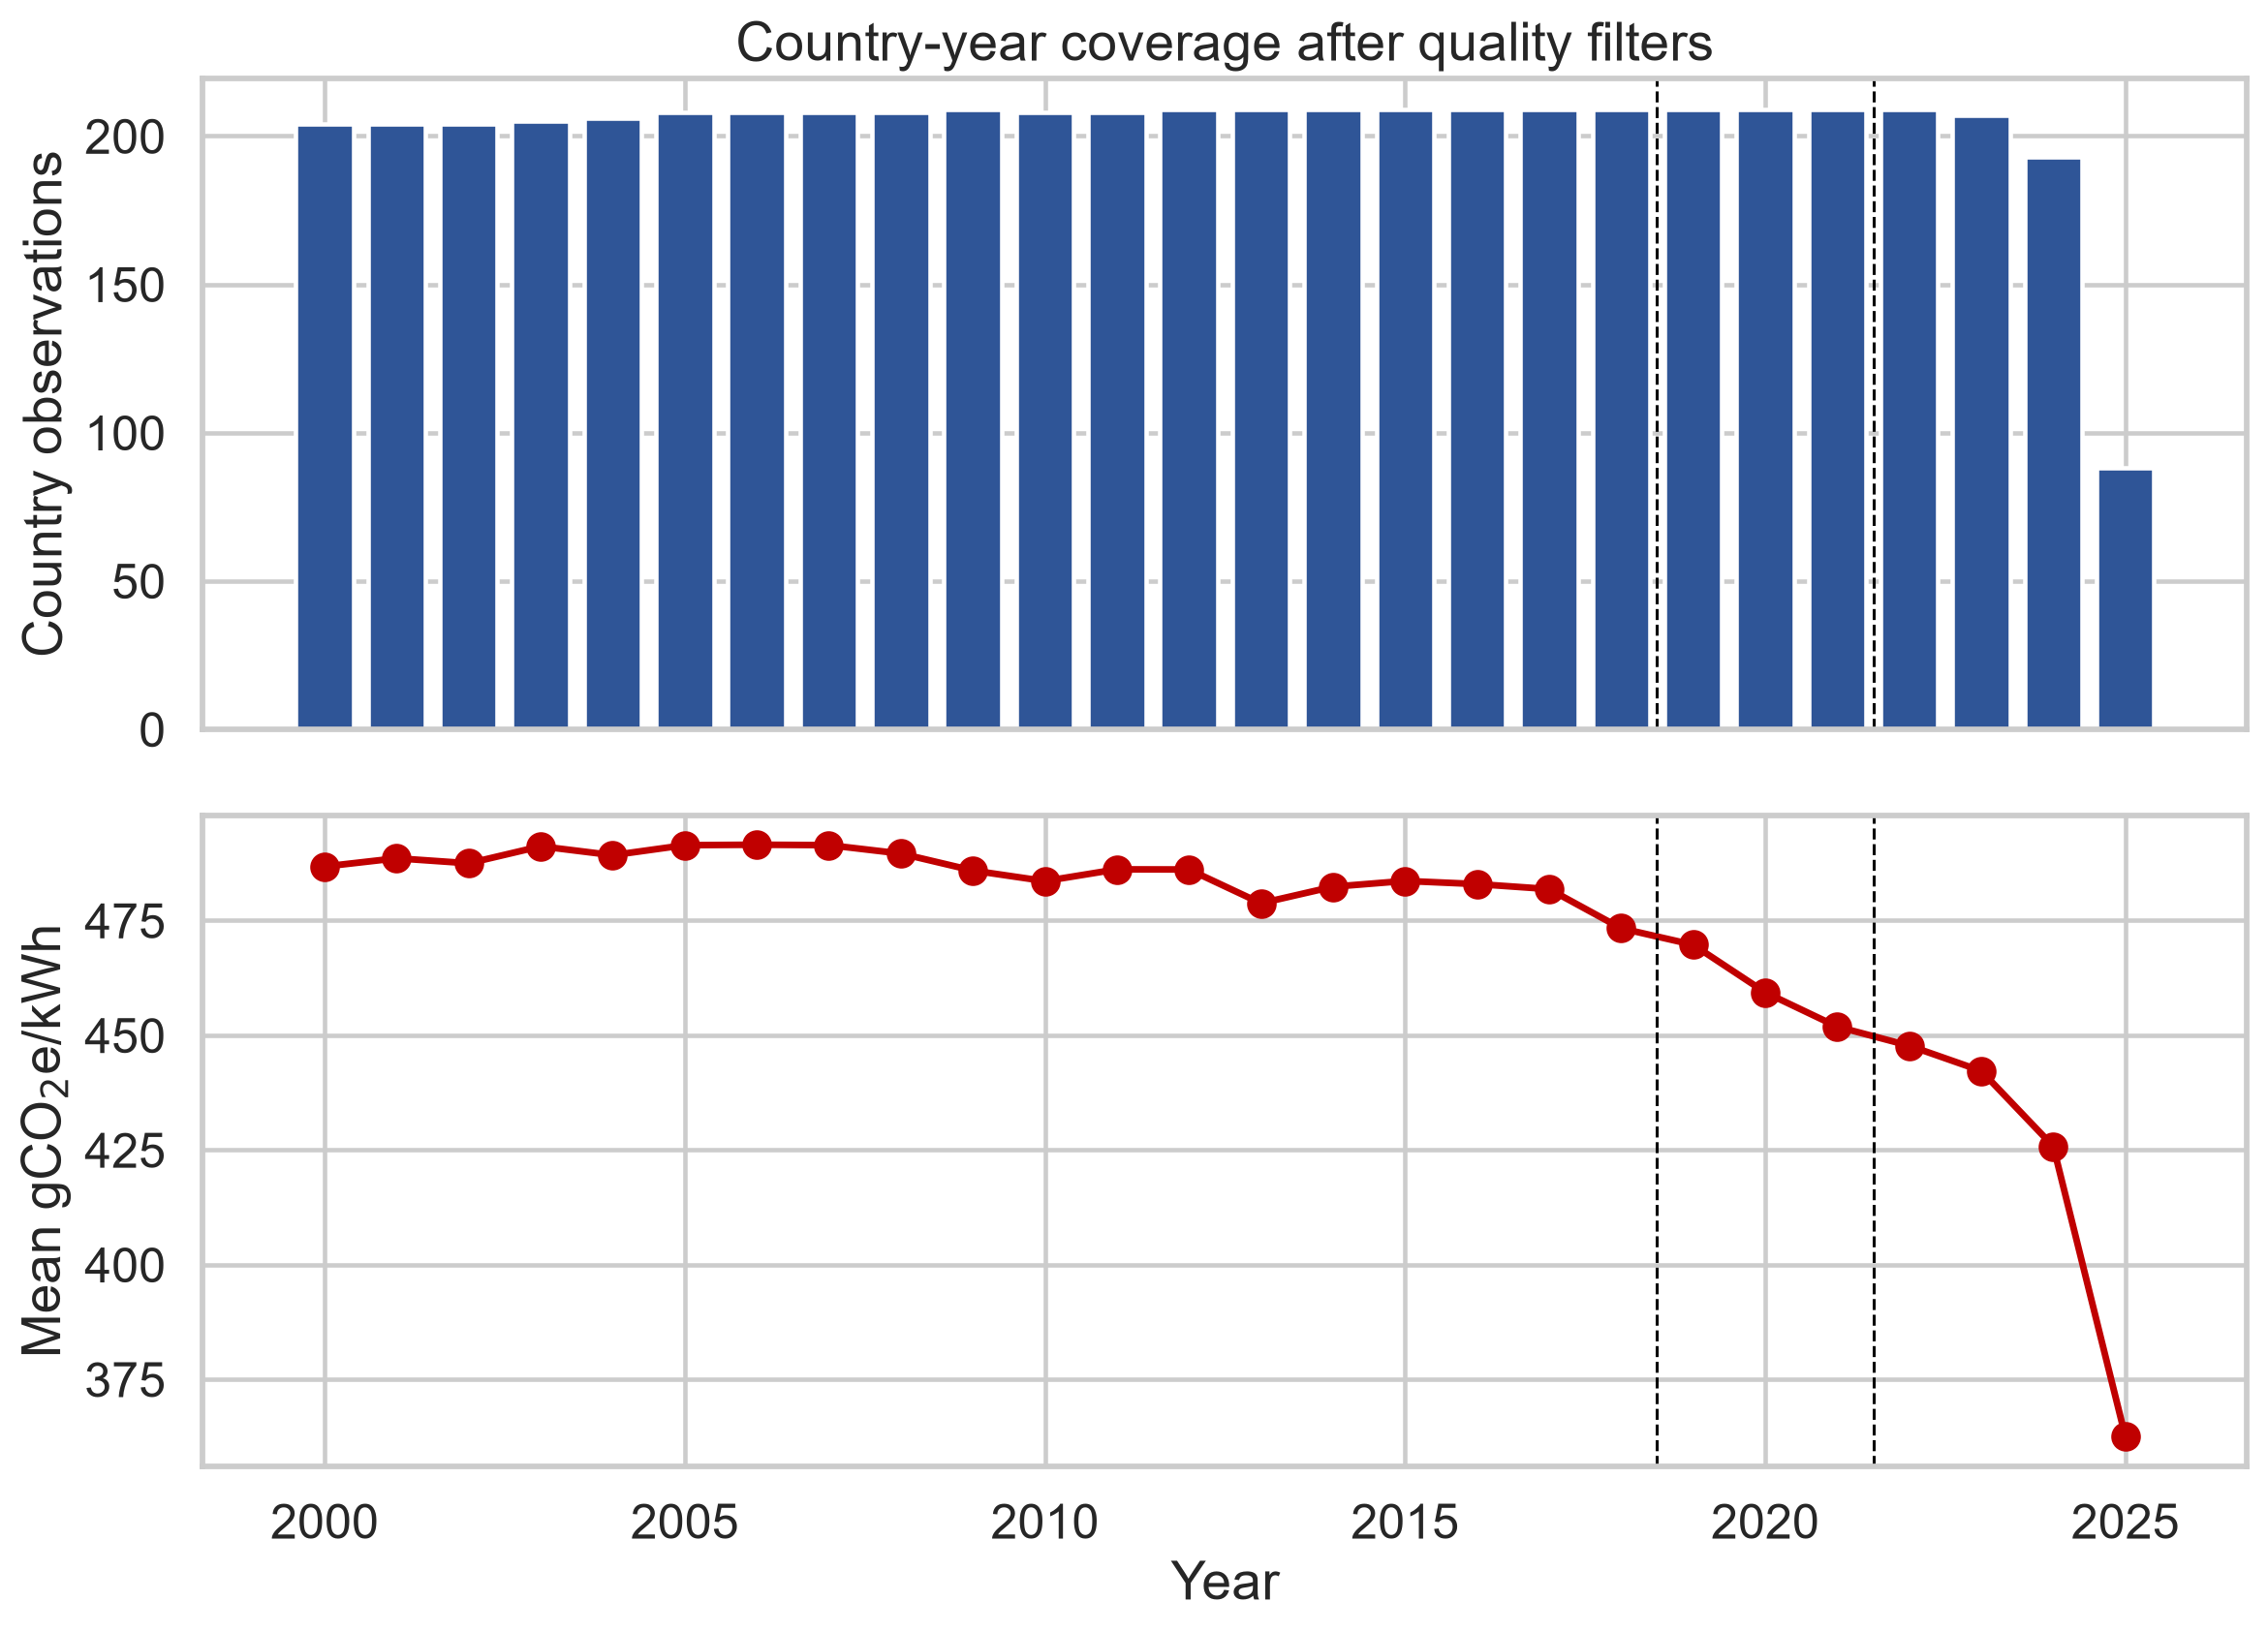
\includegraphics[width=0.92\textwidth]{panel_coverage_trend.png}
\caption{Độ phủ panel và xu hướng trung bình; đường đứt đoạn là ranh giới split.}
\end{figure}

\section{Tiền xử lý, outlier và missing}
Tỷ trọng ngoài khoảng 0--100 bị gắn thiếu; không có giá trị bất hợp lệ trong snapshot sau kiểm tra. Missing được điền median bên trong từng pipeline để tránh học thông tin test. Outlier target được đánh dấu bằng quy tắc IQR nhưng giữ lại, vì hệ thống điện có phát thải rất cao là trường hợp thực chứ không mặc nhiên là lỗi. Demand và population được biến đổi $\log(1+x)$.

\section{Leakage và đa cộng tuyến}
Các biến tổng phát thải hoặc target thay thế bị loại vì rò rỉ trực tiếp. Tổng renewables, generation và electricity per capita chỉ dùng mô tả do chồng lấn đại số với các biến chi tiết. GDP không vào đặc tả chính vì thiếu nhiều và không đủ ở phần cuối kỳ. Do tỷ trọng nguồn gần như cộng 100\%, một thành phần phải làm nhóm tham chiếu. Audit trên temporal train cho thấy chọn oil share làm tham chiếu cho VIF tối đa thấp nhất; VIF tối đa cuối cùng là 3,55.

\begin{figure}[H]
\centering
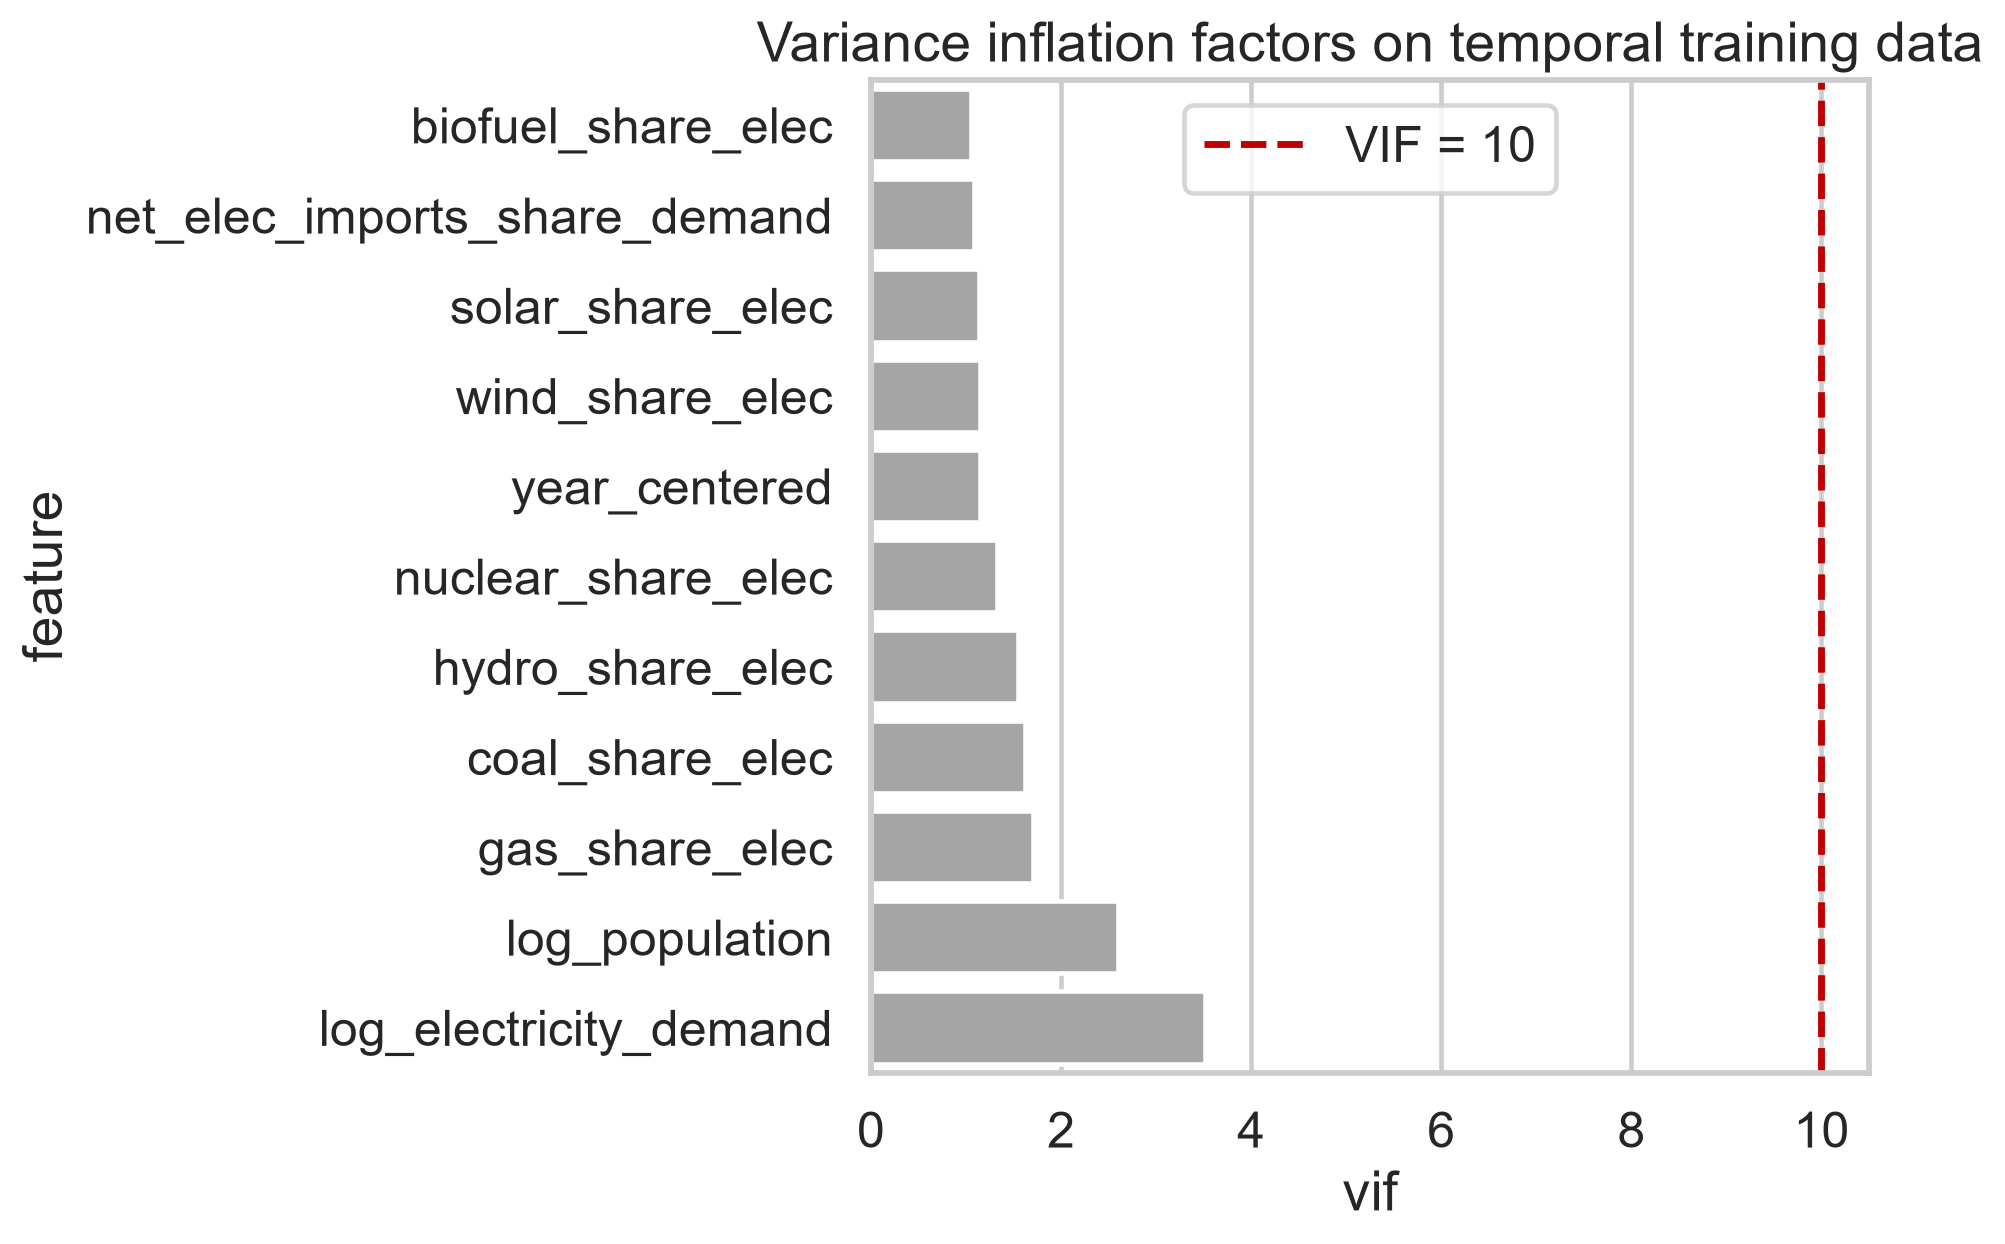
\includegraphics[width=0.84\textwidth]{vif_audit.png}
\caption{VIF của ma trận đặc trưng cuối cùng trên temporal train.}
\end{figure}

\section{Mô hình và lựa chọn siêu tham số}
Với quan sát $i,t$, bài toán là $y_{it}=f(\mathbf{x}_{it})+\epsilon_{it}$. Sáu họ mô hình được ước lượng. Tất cả cấu hình ứng viên được lưu; cấu hình có validation RMSE nhỏ nhất trong từng họ được refit trên train cộng validation rồi đánh giá test. Mô hình dùng cho XAI được chọn bằng validation temporal, không theo test.

\section{Giao thức đánh giá}
Temporal split dùng 2000--2018 để train, 2019--2021 để validation và 2022--2025 để test. Unseen-country split phân nhóm quốc gia độc quyền. Region-transfer lần lượt giữ riêng năm vùng để đánh giá trên 2022--2025 sau khi học từ các vùng còn lại đến 2021. Các metric gồm
\begin{align}
\mathrm{MAE}&=\frac{1}{n}\sum_i|y_i-\hat y_i|,\\
\mathrm{RMSE}&=\sqrt{\frac{1}{n}\sum_i(y_i-\hat y_i)^2},\\
R^2&=1-\frac{\sum_i(y_i-\hat y_i)^2}{\sum_i(y_i-\bar y)^2}.
\end{align}
Khoảng tin cậy 95\% của mô hình chính được bootstrap theo cụm quốc gia 500 lần.

\chapter{Kết quả thực nghiệm}
\section{So sánh mô hình}
\begin{figure}[H]
\centering
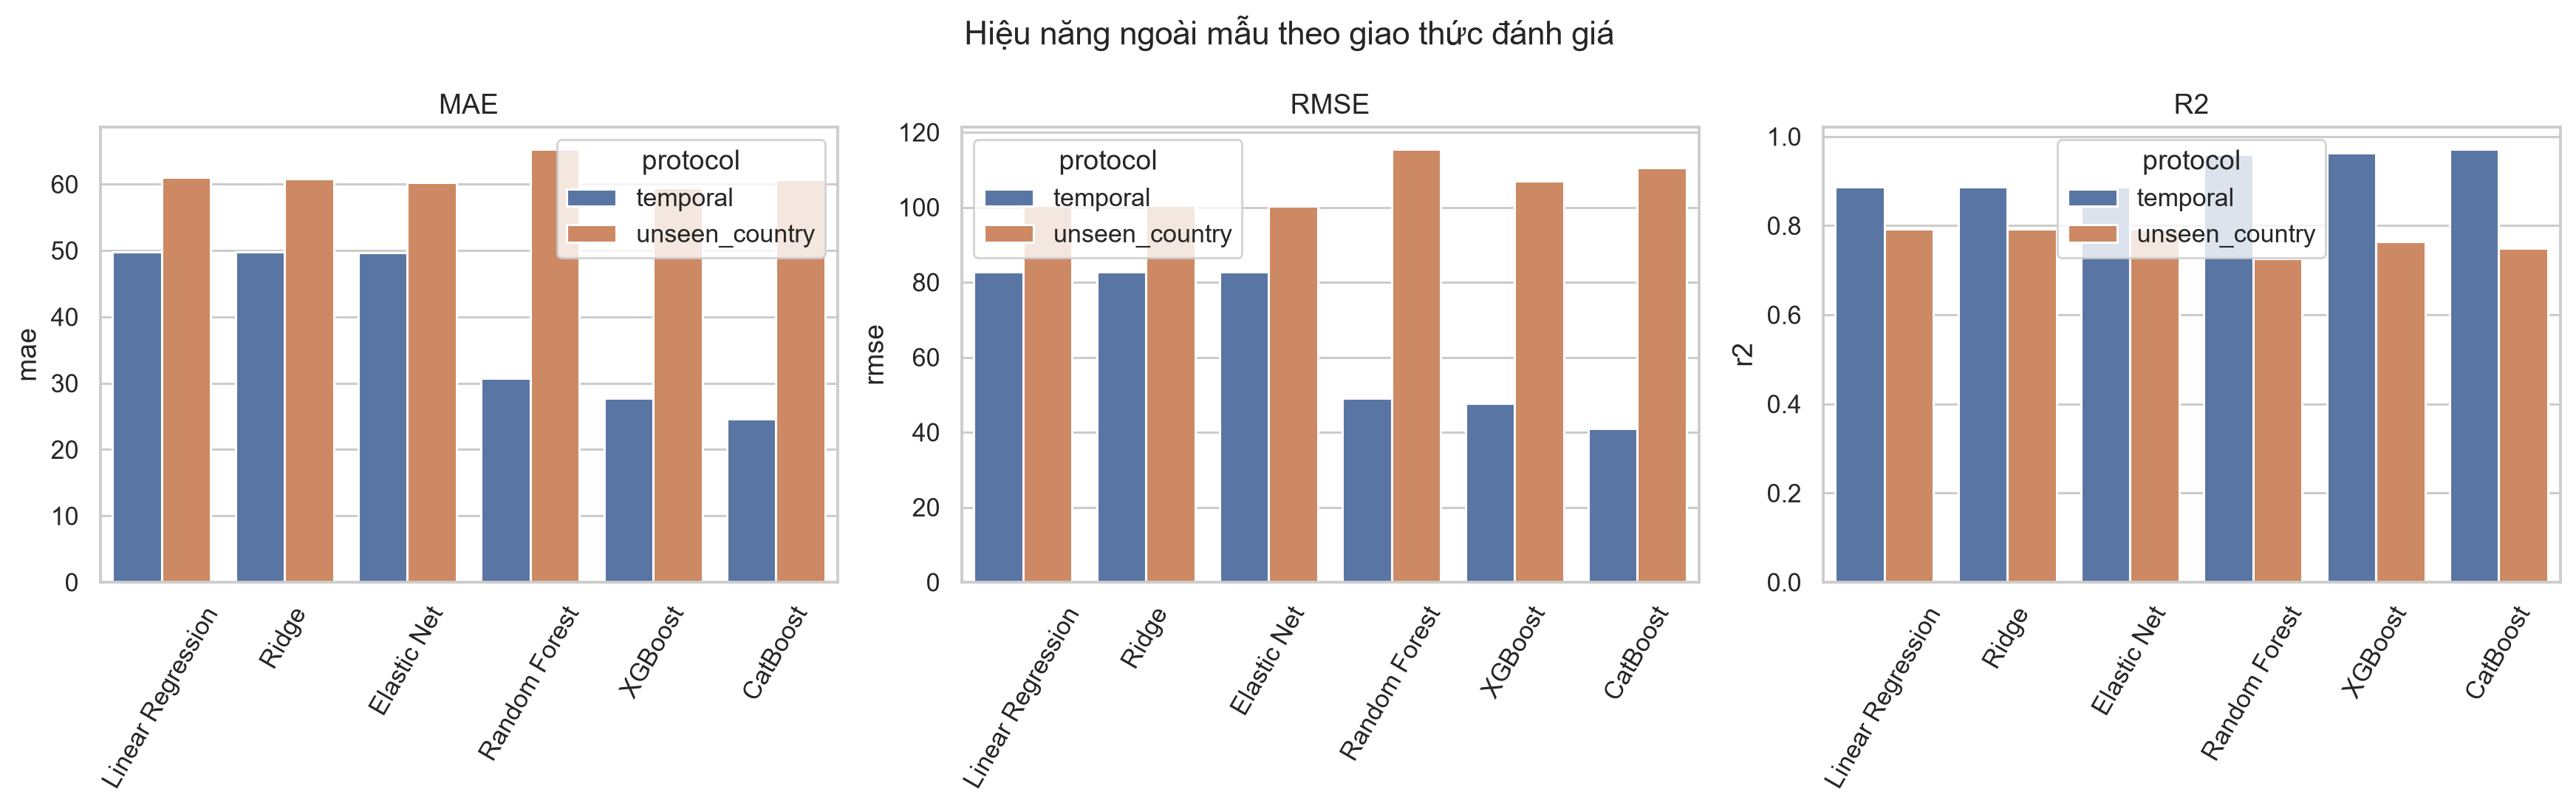
\includegraphics[width=\textwidth]{model_comparison.png}
\caption{So sánh hiệu năng ngoài mẫu theo temporal và unseen-country.}
\end{figure}

CatBoost được chọn bằng validation và đạt MAE \TemporalMAE{}, RMSE \TemporalRMSE{}, $R^2=\TemporalRsquared$ trên temporal test. Khoảng tin cậy bootstrap theo cụm quốc gia của RMSE là 27,64--44,87. Các mô hình tuyến tính có RMSE khoảng 82,5, cho thấy tương tác và phi tuyến mang thông tin đáng kể. Tuy nhiên, unseen-country khó hơn rõ rệt: CatBoost đạt MAE \UnseenMAE{}, RMSE \UnseenRMSE{} và $R^2=\UnseenRsquared$.

\small
\begin{longtable}{llrrrr}
\toprule
protocol & model\_label & n & mae & rmse & r2 \\
\midrule
\endfirsthead
\toprule
protocol & model\_label & n & mae & rmse & r2 \\
\midrule
\endhead
\midrule
\multicolumn{6}{r}{Continued on next page} \\
\midrule
\endfoot
\bottomrule
\endlastfoot
temporal & Linear Regression & 697 & 49.750000 & 82.780000 & 0.887000 \\
temporal & Ridge & 697 & 49.750000 & 82.780000 & 0.887000 \\
temporal & Elastic Net & 697 & 49.730000 & 82.780000 & 0.887000 \\
temporal & Random Forest & 697 & 30.700000 & 49.050000 & 0.960000 \\
temporal & XGBoost & 697 & 27.720000 & 47.690000 & 0.962000 \\
temporal & CatBoost & 697 & 24.680000 & 41.040000 & 0.972000 \\
unseen\_country & Linear Regression & 1047 & 61.060000 & 100.590000 & 0.792000 \\
unseen\_country & Ridge & 1047 & 60.820000 & 100.530000 & 0.792000 \\
unseen\_country & Elastic Net & 1047 & 60.270000 & 100.380000 & 0.793000 \\
unseen\_country & Random Forest & 1047 & 65.320000 & 115.550000 & 0.726000 \\
unseen\_country & XGBoost & 1047 & 59.490000 & 107.070000 & 0.764000 \\
unseen\_country & CatBoost & 1047 & 60.700000 & 110.610000 & 0.749000 \\
\end{longtable}

\normalsize

\section{Chuyển giao vùng}
\begin{figure}[H]
\centering
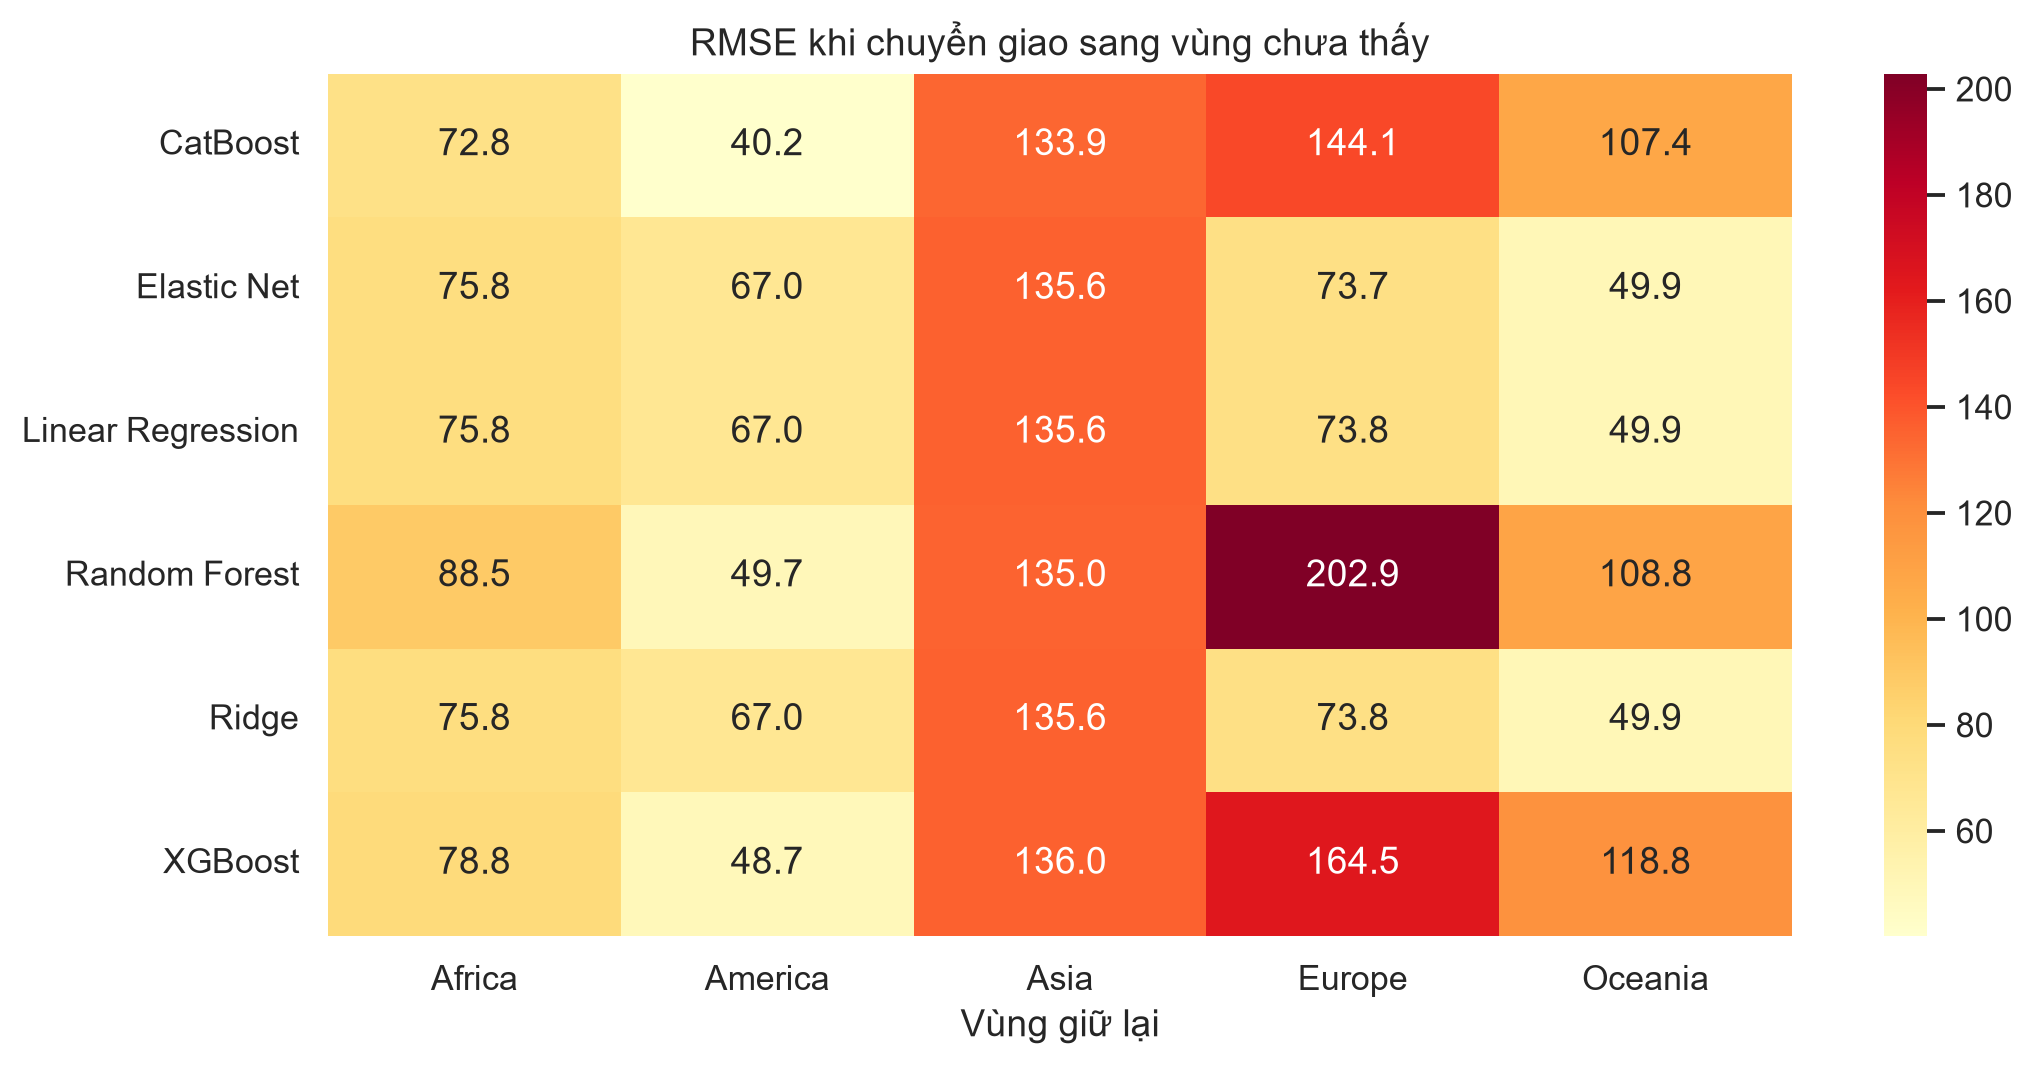
\includegraphics[width=0.92\textwidth]{region_transfer_rmse.png}
\caption{RMSE khi giữ lại từng vùng và dự báo giai đoạn 2022--2025.}
\end{figure}

Không có một họ mô hình thắng ở mọi vùng. RMSE tốt nhất theo vùng lần lượt là 74,70 ở Africa (Elastic Net), 41,09 ở America (CatBoost), 136,10 ở Asia (Linear Regression), 74,52 ở Europe (Elastic Net) và 47,61 ở Oceania (Linear Regression). Kết quả cho thấy mô hình cây mạnh trong nội suy thời gian nhưng có thể ngoại suy kém khi toàn bộ vùng bị giữ lại.

\section{Explainable AI}
\begin{figure}[H]
\centering
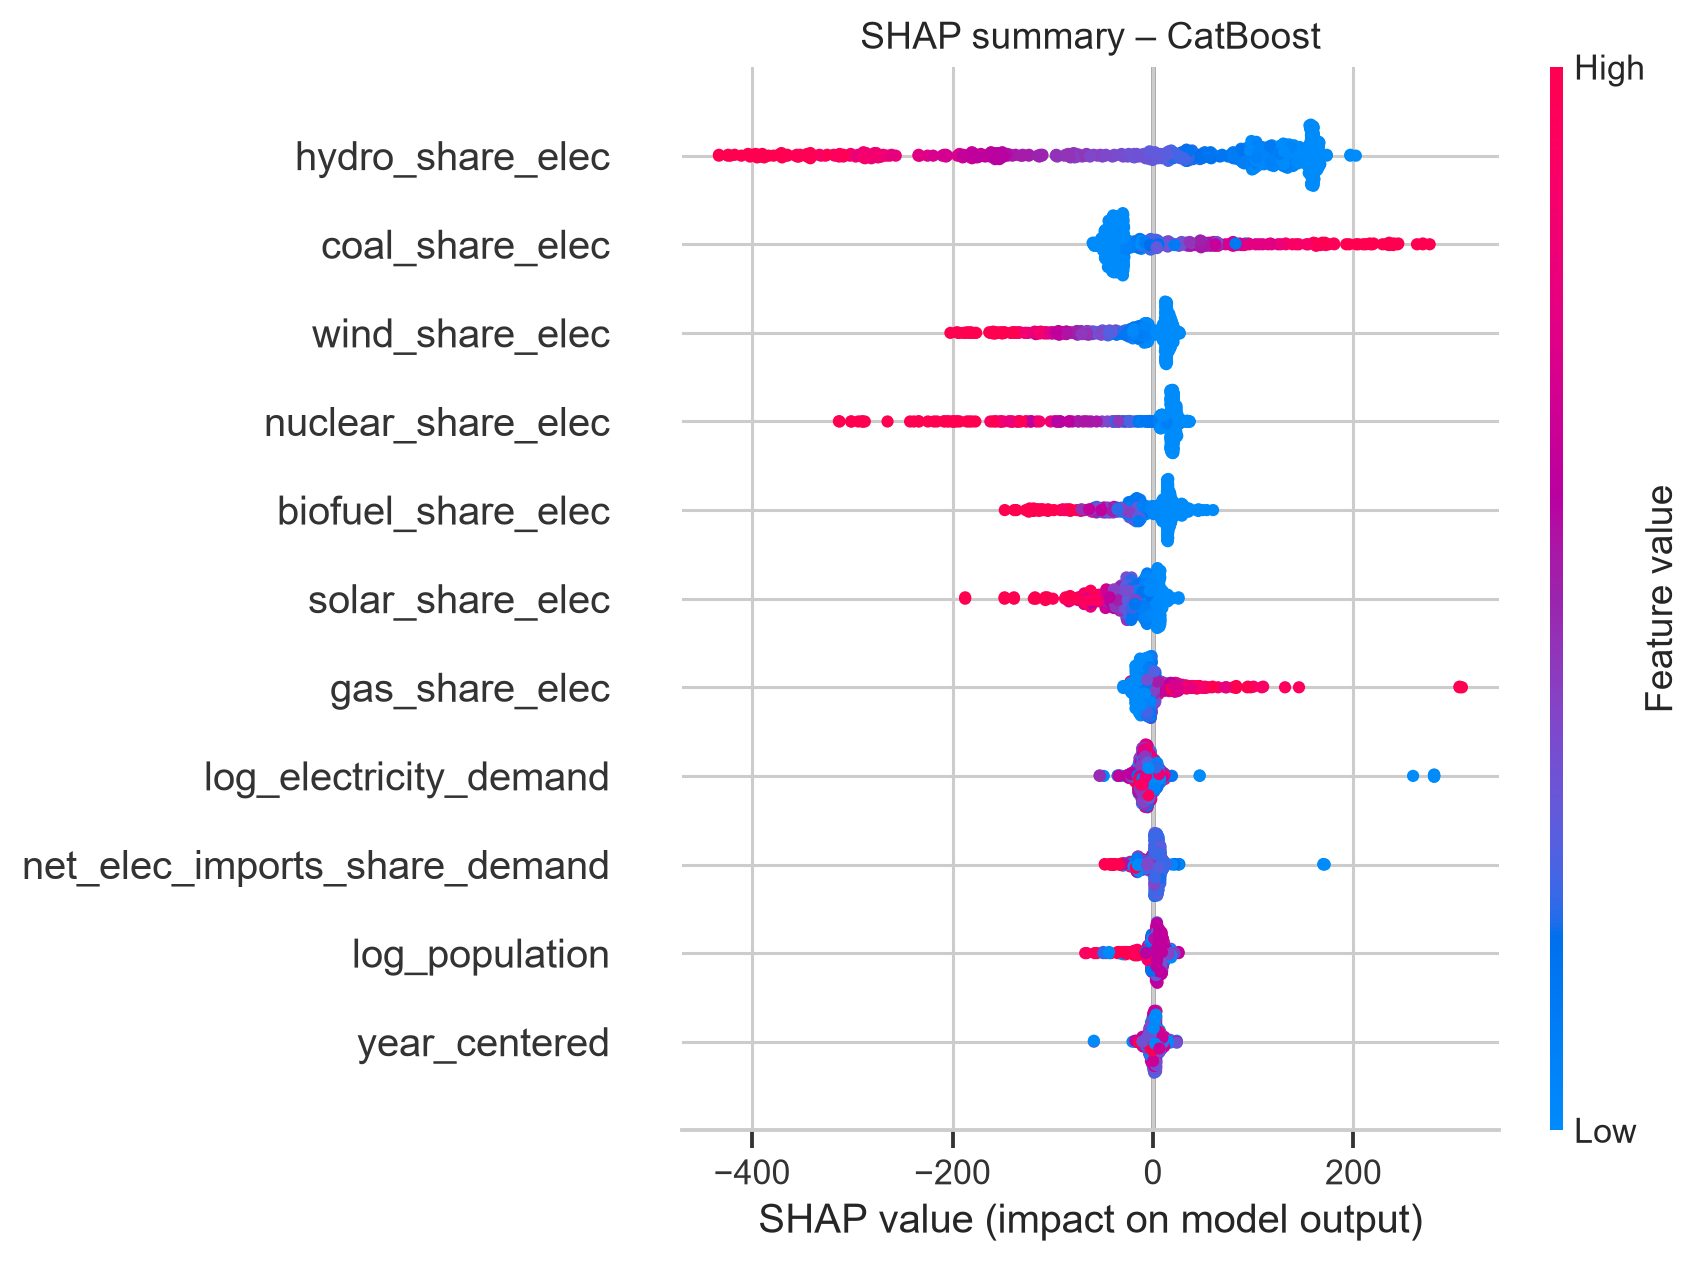
\includegraphics[width=0.95\textwidth]{shap_summary.png}
\caption{Phân bố đóng góp SHAP của mô hình CatBoost được chọn.}
\end{figure}

Theo mean absolute SHAP, hydro share đứng đầu (141,41), tiếp theo là coal (44,13), wind (34,88), nuclear (33,02), biofuel (25,17) và solar (23,95). Dấu của từng điểm SHAP phải được đọc cùng mức đặc trưng và nền dữ liệu; không nên diễn giải mean SHAP đơn lẻ như hệ số.

\begin{figure}[H]
\centering
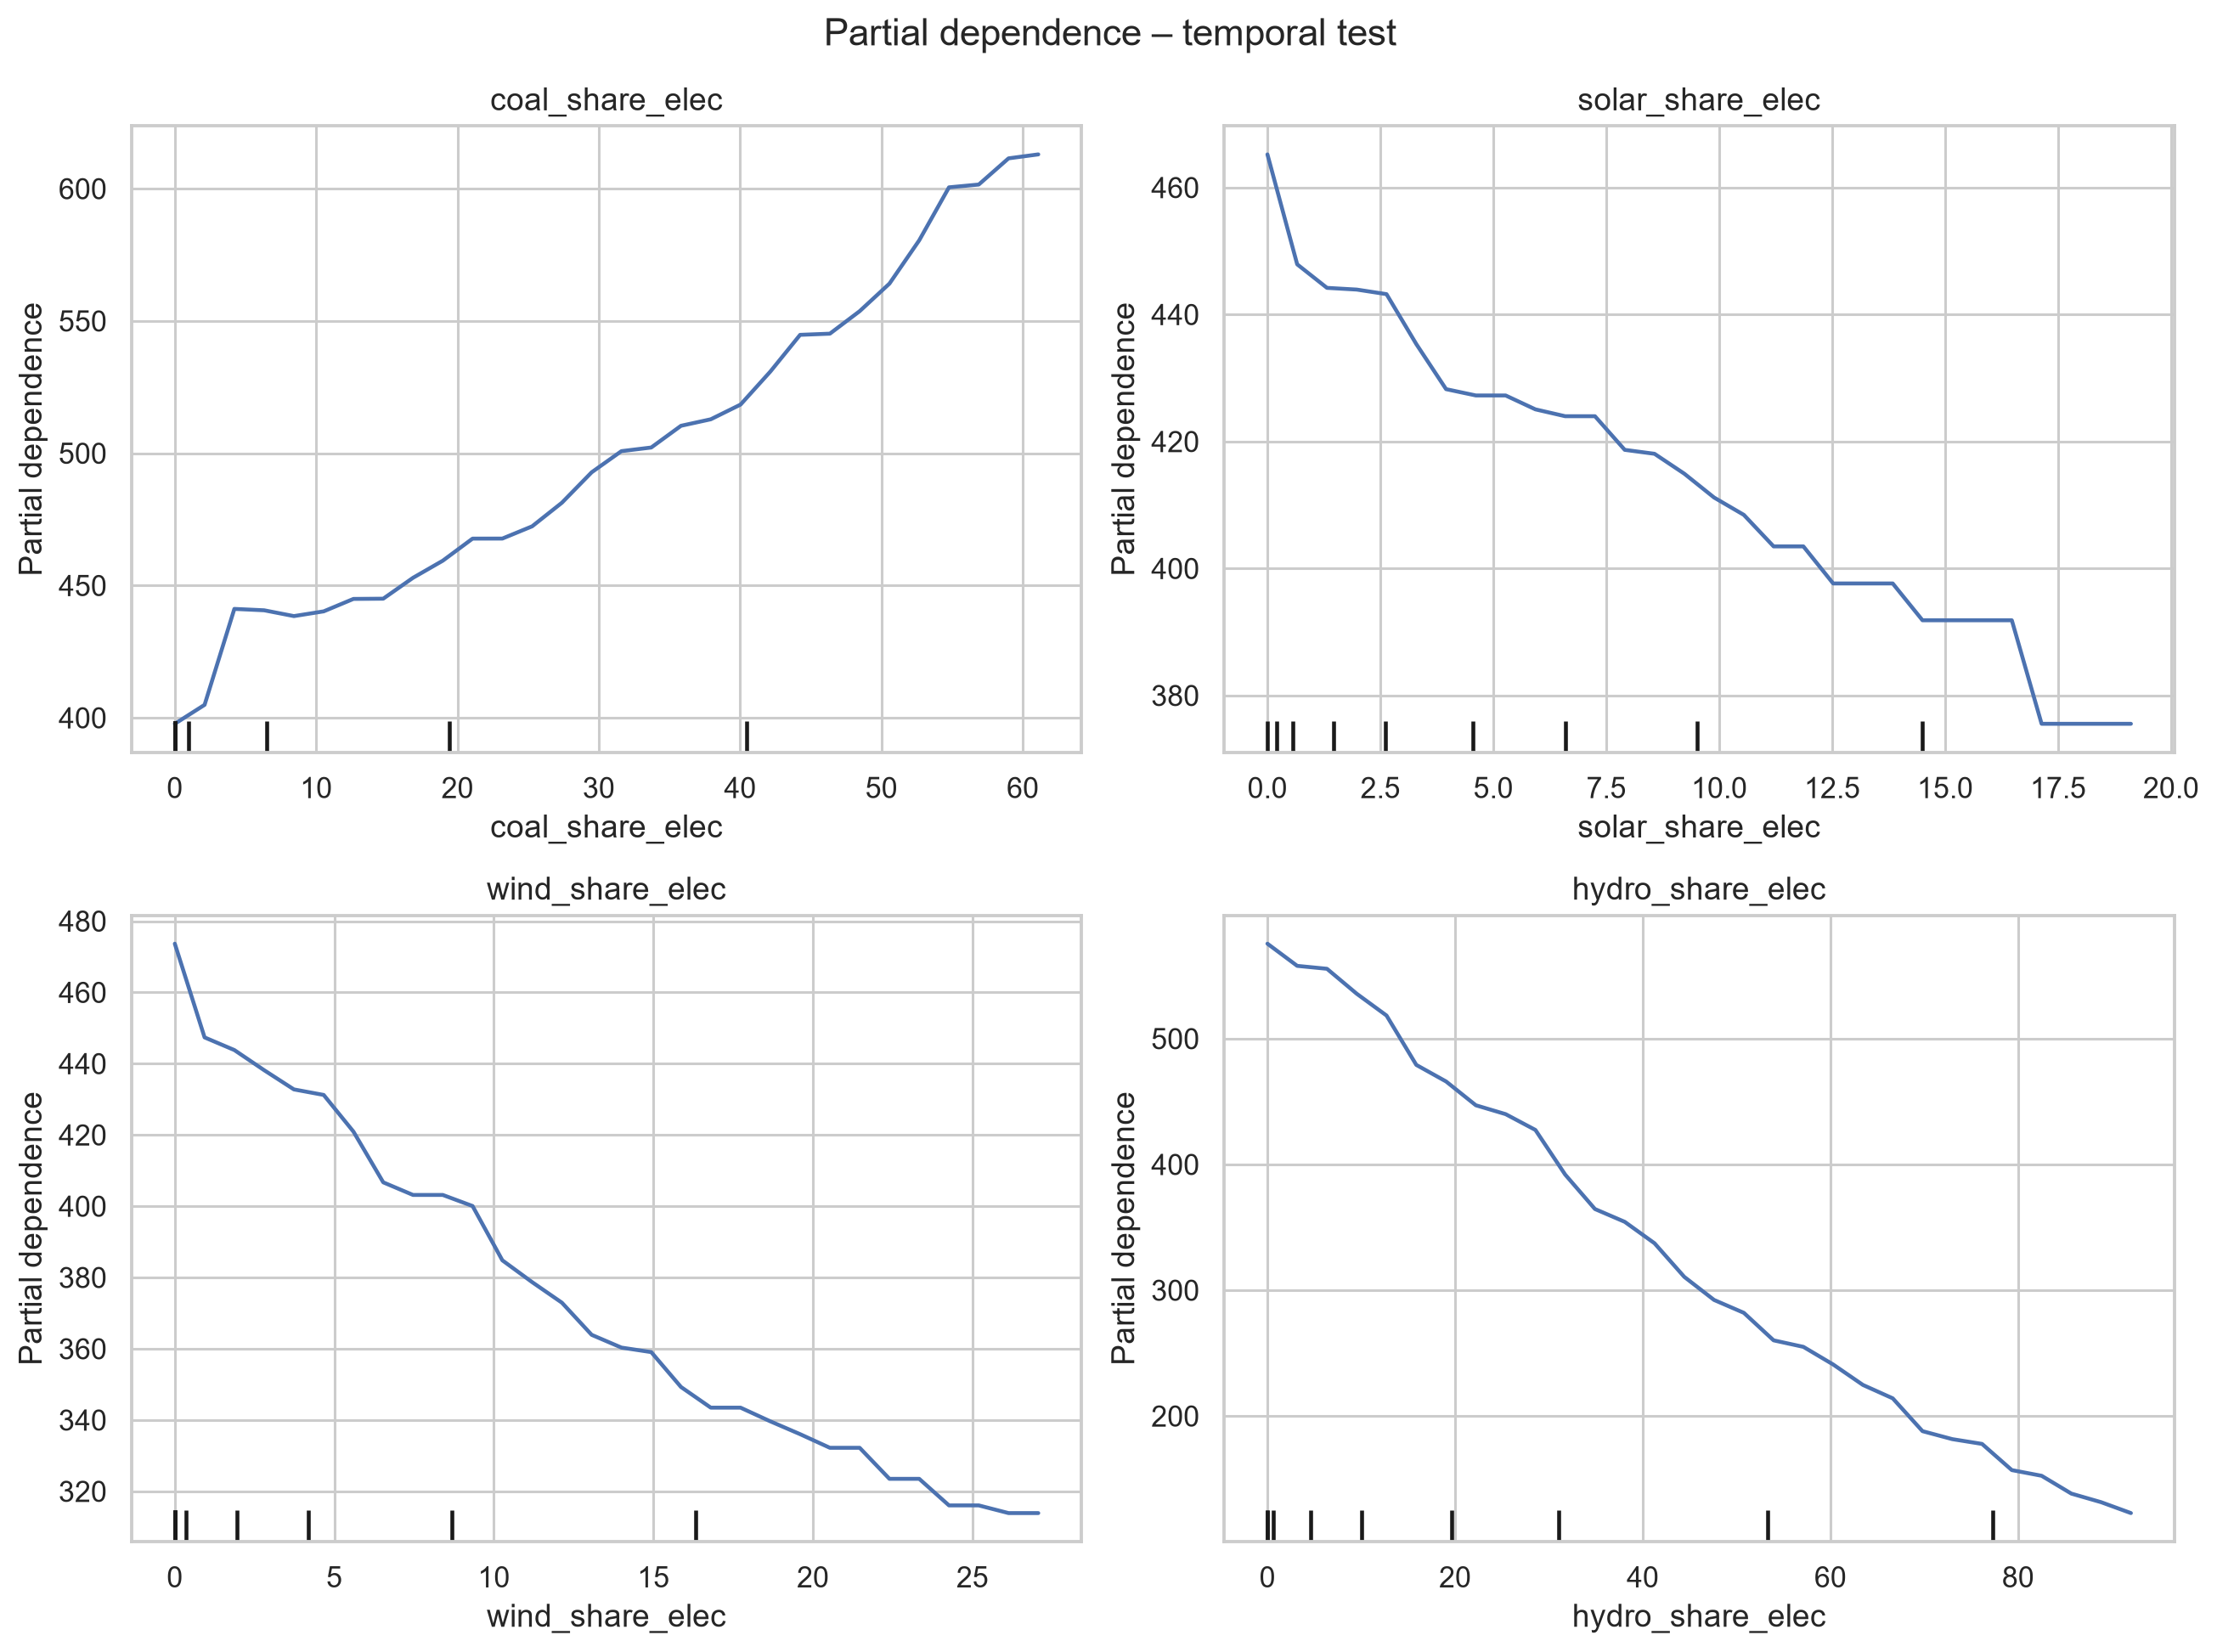
\includegraphics[width=0.95\textwidth]{partial_dependence.png}
\caption{Partial dependence của bốn thành phần cơ cấu nguồn điện.}
\end{figure}

Permutation importance kiểm tra vai trò dự báo trực tiếp trên temporal test, còn partial dependence cho thấy phản ứng trung bình phi tuyến. Sự thống nhất tương đối giữa các công cụ làm tăng độ tin cậy về cấu trúc hàm dự báo, nhưng tương quan giữa các tỷ trọng vẫn đòi hỏi thận trọng.

\section{Dị biệt và phân tích sai số}
\begin{figure}[H]
\centering
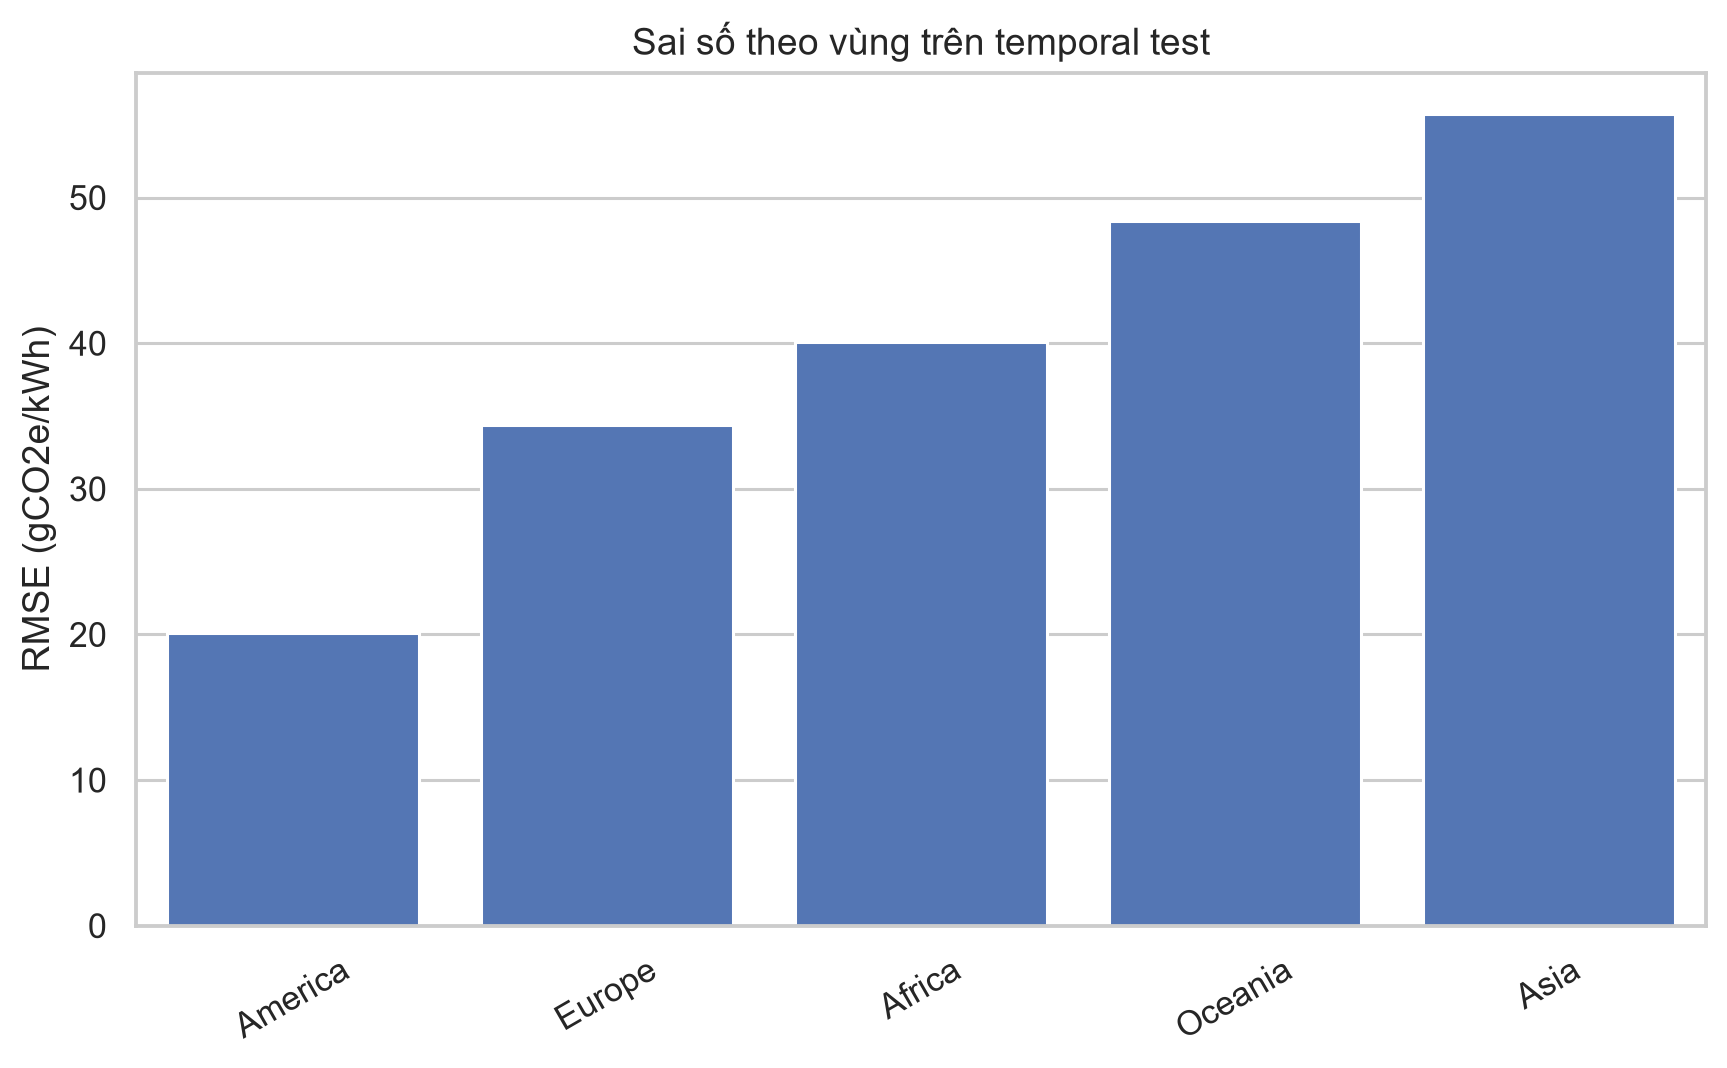
\includegraphics[width=0.82\textwidth]{heterogeneity_region.png}
\caption{RMSE temporal test của mô hình chính theo vùng.}
\end{figure}

Sai số không đồng nhất giữa vùng và nhóm nguồn chi phối. Đây là bằng chứng chống lại việc chỉ báo cáo một metric toàn cục. File \texttt{heterogeneity\_metrics.csv} và \texttt{largest\_errors.csv} cho phép truy vết nhóm và quan sát có sai số lớn nhất.

\chapter{Nghiên cứu tình huống Việt Nam}
\section{Dự báo ngoài mẫu}
\begin{figure}[H]
\centering
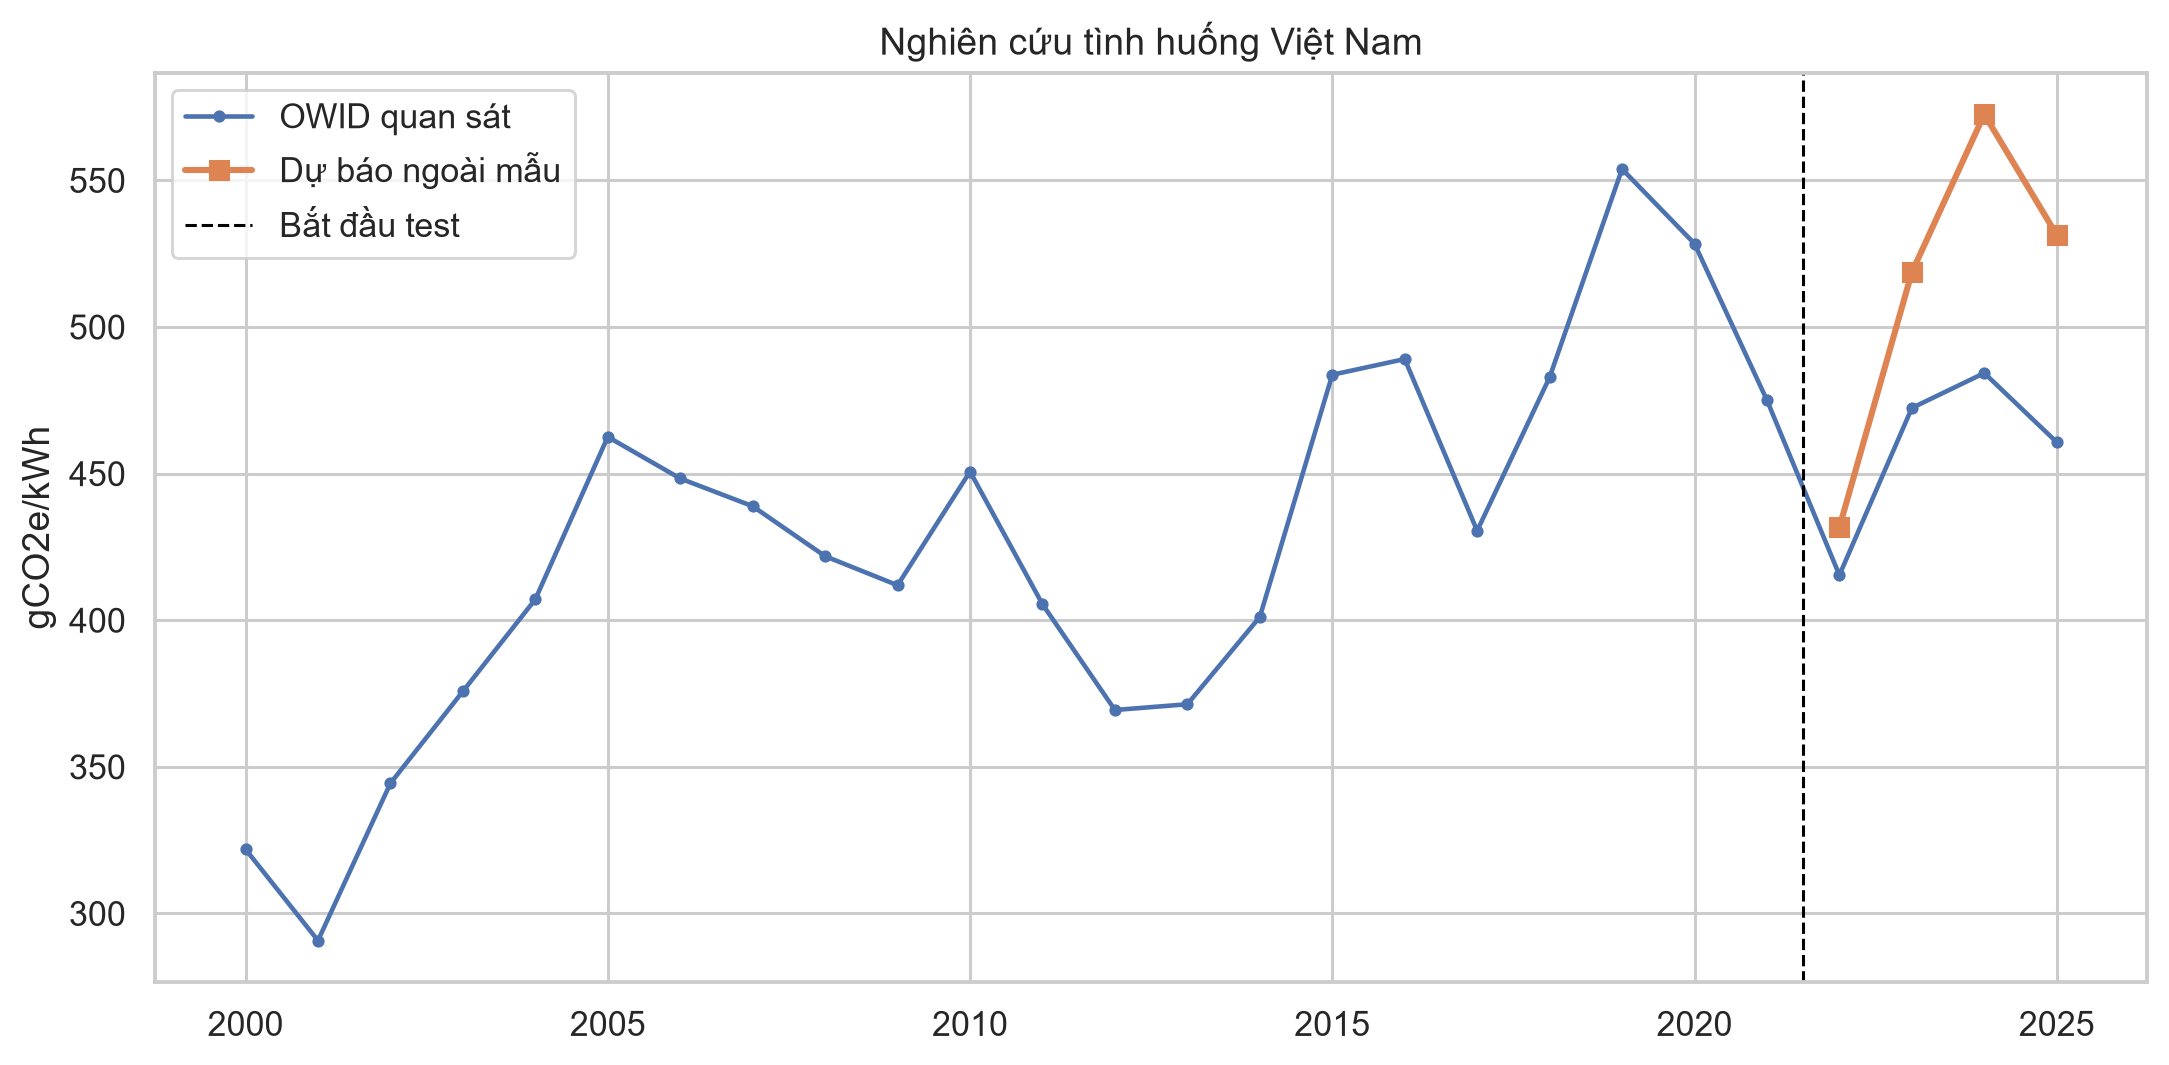
\includegraphics[width=0.94\textwidth]{vietnam_case.png}
\caption{Quan sát OWID và dự báo ngoài mẫu cho Việt Nam.}
\end{figure}

Trong năm \VietnamLatestYear, cường độ carbon quan sát của Việt Nam là \VietnamActual{} gCO$_2$e/kWh và dự báo CatBoost là \VietnamPredicted{}. Sai số dương 39,89 gCO$_2$e/kWh cho thấy cần giữ bất định ở cấp quốc gia ngay cả khi hiệu năng toàn cục cao.

\section{Kịch bản cơ cấu điện}
Các kịch bản bắt đầu từ hàng Việt Nam năm 2025 và chỉ thay đổi các tỷ trọng nêu trong tên, giữ demand, population, imports và year cố định. Vì mô hình không phải thiết kế nhân quả, kết quả chỉ mô tả phản ứng của hàm dự báo.

\begin{figure}[H]
\centering
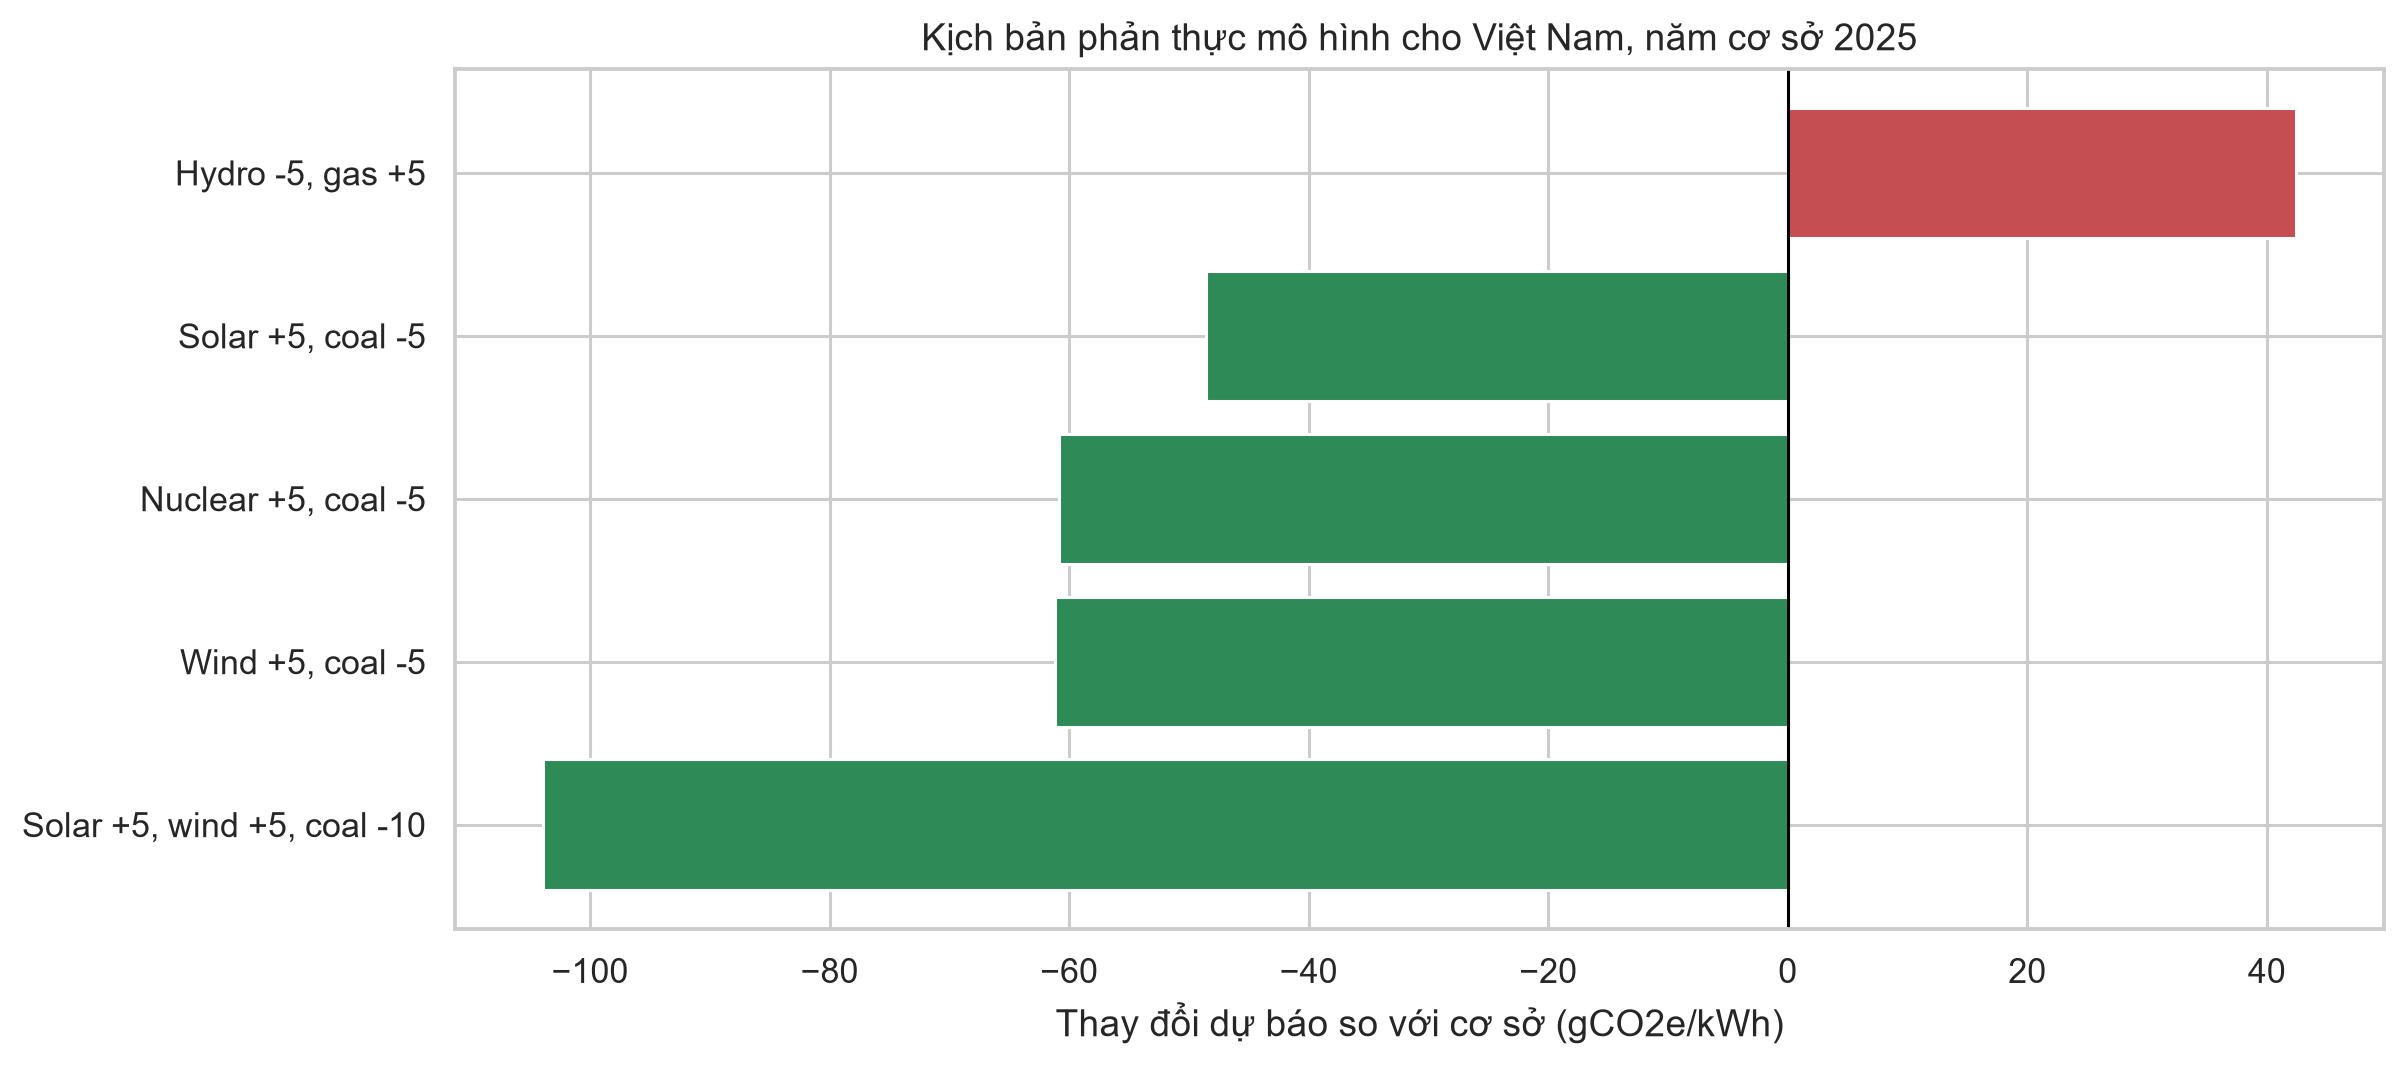
\includegraphics[width=0.95\textwidth]{vietnam_scenarios.png}
\caption{Thay đổi dự báo CatBoost dưới các kịch bản cơ cấu điện của Việt Nam.}
\end{figure}

Kịch bản giảm 10 điểm phần trăm than và tăng đồng thời 5 điểm mặt trời, 5 điểm gió cho mức giảm dự báo lớn nhất, \BestScenarioDelta{} gCO$_2$e/kWh. Kịch bản giảm 5 điểm thủy điện và tăng 5 điểm khí làm dự báo tăng 36,84 gCO$_2$e/kWh. Đây là so sánh ceteris paribus, chưa xét ràng buộc lưới, lưu trữ, chi phí, độ tin cậy hay diễn biến nhu cầu.

\small
\begin{tabular}{p{6.2cm}rrr}
\toprule
Kịch bản & Dự báo & Thay đổi & Thay đổi pct \\
\midrule
Quan sát cơ sở & 531.420000 & 0.000000 & 0.000000 \\
Solar +5, coal -5 & 482.850000 & -48.570000 & -9.140000 \\
Wind +5, coal -5 & 470.290000 & -61.130000 & -11.500000 \\
Solar +5, wind +5, coal -10 & 427.480000 & -103.940000 & -19.560000 \\
Nuclear +5, coal -5 & 470.570000 & -60.860000 & -11.450000 \\
Hydro -5, gas +5 & 573.880000 & 42.460000 & 7.990000 \\
\bottomrule
\end{tabular}

\normalsize

\chapter{Thảo luận}
\section{Hàm ý học thuật}
Kết quả temporal cho thấy boosting mô tả tốt quan hệ phi tuyến giữa cơ cấu nguồn và cường độ carbon. Khoảng cách lớn giữa temporal và unseen-country cho thấy độ chính xác khi dự báo tương lai của các quốc gia đã thấy không bảo đảm khả năng chuyển sang quốc gia mới. Region-transfer củng cố nhận định này: mô hình tuyến tính điều chuẩn có thể ổn định hơn cây ở một số miền ngoại suy.

\section{Hàm ý thực tiễn}
Mô hình và XAI phù hợp để sàng lọc kịch bản, phát hiện trường hợp bất thường và định lượng sơ bộ sự dịch chuyển trong không gian đặc trưng quan sát. Với Việt Nam, giảm than đồng thời tăng nguồn carbon thấp liên quan đến mức cường độ dự báo thấp hơn. Tuy vậy, quyết định quy hoạch cần kết hợp mô hình hệ thống điện, chi phí, công suất khả dụng, truyền tải, lưu trữ và an ninh năng lượng.

\section{Hạn chế}
Thứ nhất, target và feature cùng năm làm đây là mô hình hóa/nowcasting, không phải dự báo nhiều năm trước. Thứ hai, dữ liệu quốc gia che lấp dị biệt theo giờ và vùng lưới. Thứ ba, missing được impute và độ phủ năm 2025 có thể thay đổi. Thứ tư, SHAP và PDP chịu ảnh hưởng của tương quan đặc trưng. Thứ năm, không có thiết kế nhận dạng nhân quả, nên scenario không ước lượng tác động chính sách.

\section{Hướng nghiên cứu tiếp theo}
Nghiên cứu tiếp theo nên bổ sung dữ liệu theo giờ, biến giá nhiên liệu, thời tiết, liên kết lưới và công suất lưu trữ; dùng compositional data analysis; mô hình phân cấp theo vùng; conformal prediction; và đánh giá backtesting theo nhiều cửa sổ thời gian. Với Việt Nam, có thể ghép mô hình dự báo với tối ưu hóa hệ thống điện và các kịch bản quy hoạch chính thức.

\chapter{Kết luận}
Luận văn đã xây dựng một workflow end-to-end, tái lập và có khả năng giải thích cho cường độ carbon điện của \PanelCountries{} quốc gia đến năm \PanelEndYear. CatBoost cho hiệu năng temporal tốt nhất theo tiêu chí lựa chọn đã khóa, nhưng mức suy giảm ở unseen-country và region-transfer cho thấy tổng quát hóa không gian khó hơn tổng quát hóa thời gian. SHAP, permutation importance và PDP nhất quán rằng cơ cấu nguồn là trung tâm của hàm dự báo. Case study Việt Nam chứng minh giá trị thăm dò của mô hình đồng thời xác lập ranh giới: kết quả kịch bản là phản thực mô hình, không phải kết luận nhân quả. Notebook có output, bảng CSV, model, figure, manifest và LaTeX tạo thành chuỗi bằng chứng có thể kiểm tra độc lập.

\begin{thebibliography}{99}
\bibitem{owidcarbon} Our World in Data. \textit{Carbon intensity of electricity}. Ember (2026), processed by OWID. \url{https://ourworldindata.org/grapher/carbon-intensity-electricity}.
\bibitem{owidenergy} Our World in Data. \textit{Energy Data}. \url{https://github.com/owid/energy-data}.
\bibitem{hoerl1970} A. E. Hoerl and R. W. Kennard. Ridge Regression: Biased Estimation for Nonorthogonal Problems. \textit{Technometrics}, 12(1), 1970. doi:10.1080/00401706.1970.10488634.
\bibitem{zou2005} H. Zou and T. Hastie. Regularization and Variable Selection via the Elastic Net. \textit{JRSS B}, 67(2), 2005. doi:10.1111/j.1467-9868.2005.00503.x.
\bibitem{breiman2001} L. Breiman. Random Forests. \textit{Machine Learning}, 45, 2001. doi:10.1023/A:1010933404324.
\bibitem{chen2016} T. Chen and C. Guestrin. XGBoost: A Scalable Tree Boosting System. \textit{KDD}, 2016. doi:10.1145/2939672.2939785.
\bibitem{prokhorenkova2018} L. Prokhorenkova et al. CatBoost: unbiased boosting with categorical features. \textit{NeurIPS}, 2018.
\bibitem{lundberg2017} S. M. Lundberg and S.-I. Lee. A Unified Approach to Interpreting Model Predictions. \textit{NeurIPS}, 2017.
\bibitem{aras2022} S. Aras and M. H. Van. Explainable artificial intelligence for energy use and CO$_2$ emissions. \textit{Applied Energy}, 328, 120163, 2022. doi:10.1016/j.apenergy.2022.120163.
\bibitem{dayahead2023} \textit{Day-ahead carbon intensity forecasting with machine learning}. \textit{Engineering Applications of Artificial Intelligence}, 2023. doi:10.1016/j.engappai.2023.106314.
\end{thebibliography}

\appendix
\chapter{Bảng kết quả bổ sung}
\section{Khoảng tin cậy bootstrap}
\begin{tabular}{lrrrr}
\toprule
metric & estimate & ci\_low & ci\_high & bootstrap\_repetitions \\
\midrule
mae & 24.675000 & 20.868000 & 29.033000 & 500 \\
rmse & 41.041000 & 31.020000 & 51.177000 & 500 \\
r2 & 0.972000 & 0.958000 & 0.983000 & 500 \\
\bottomrule
\end{tabular}


\section{Kết quả region-transfer đầy đủ}
\small
\begin{longtable}{llrrrr}
\toprule
held\_out\_region & model\_label & test\_n & mae & rmse & r2 \\
\midrule
\endfirsthead
\toprule
held\_out\_region & model\_label & test\_n & mae & rmse & r2 \\
\midrule
\endhead
\midrule
\multicolumn{6}{r}{Continued on next page} \\
\midrule
\endfoot
\bottomrule
\endlastfoot
Africa & Linear Regression & 168 & 50.560000 & 75.814000 & 0.901000 \\
Africa & Ridge & 168 & 50.559000 & 75.814000 & 0.901000 \\
Africa & Elastic Net & 168 & 50.522000 & 75.796000 & 0.901000 \\
Africa & Random Forest & 168 & 60.967000 & 88.508000 & 0.865000 \\
Africa & XGBoost & 168 & 57.862000 & 78.752000 & 0.893000 \\
Africa & CatBoost & 168 & 51.912000 & 72.803000 & 0.909000 \\
America & Linear Regression & 147 & 36.437000 & 67.045000 & 0.920000 \\
America & Ridge & 147 & 36.437000 & 67.045000 & 0.920000 \\
America & Elastic Net & 147 & 36.414000 & 67.037000 & 0.920000 \\
America & Random Forest & 147 & 32.191000 & 49.680000 & 0.956000 \\
America & XGBoost & 147 & 33.227000 & 48.705000 & 0.958000 \\
America & CatBoost & 147 & 28.973000 & 40.185000 & 0.971000 \\
Asia & Linear Regression & 176 & 70.430000 & 135.565000 & 0.691000 \\
Asia & Ridge & 176 & 70.430000 & 135.565000 & 0.691000 \\
Asia & Elastic Net & 176 & 70.443000 & 135.574000 & 0.691000 \\
Asia & Random Forest & 176 & 78.265000 & 134.994000 & 0.694000 \\
Asia & XGBoost & 176 & 73.549000 & 135.997000 & 0.689000 \\
Asia & CatBoost & 176 & 70.223000 & 133.880000 & 0.699000 \\
Europe & Linear Regression & 160 & 58.914000 & 73.768000 & 0.881000 \\
Europe & Ridge & 160 & 58.914000 & 73.768000 & 0.881000 \\
Europe & Elastic Net & 160 & 58.866000 & 73.737000 & 0.881000 \\
Europe & Random Forest & 160 & 163.652000 & 202.877000 & 0.097000 \\
Europe & XGBoost & 160 & 133.700000 & 164.460000 & 0.407000 \\
Europe & CatBoost & 160 & 120.098000 & 144.124000 & 0.544000 \\
Oceania & Linear Regression & 46 & 37.225000 & 49.901000 & 0.914000 \\
Oceania & Ridge & 46 & 37.225000 & 49.901000 & 0.914000 \\
Oceania & Elastic Net & 46 & 37.238000 & 49.920000 & 0.914000 \\
Oceania & Random Forest & 46 & 65.889000 & 108.845000 & 0.590000 \\
Oceania & XGBoost & 46 & 67.770000 & 118.783000 & 0.512000 \\
Oceania & CatBoost & 46 & 56.951000 & 107.399000 & 0.601000 \\
\end{longtable}

\normalsize

\chapter{Tái lập nghiên cứu}
Notebook chuẩn là \texttt{notebooks/Explainable\_Carbon\_Intensity\_Thesis.ipynb}. Lệnh \texttt{run\_all.ps1} cài dependency, kiểm tra/tải dữ liệu, chạy notebook và biên dịch XeLaTeX. Mọi số trong tài liệu này xuất phát từ \texttt{outputs/thesis/tables}; không có bảng kết quả định lượng được nhập độc lập.

\end{document}
